\documentclass[11pt]{article}
\usepackage[margin=1in]{geometry}
\usepackage{graphicx}
\usepackage{amsmath}
\usepackage{amssymb}
\usepackage{float}
\usepackage{subcaption}

\title{Work Type Summary Statistics}

\begin{document}
\maketitle

\section{Work Type Overview}
  Judge calendar assignments generally have an acronym indicating the type of the assignment (e.g. Marion GS). There are eight different assignment types, each with a corresponding acronym. Assignments can have more than one type (e.g. Marion GS CC). Our study focuses on criminal cases, which are heard in general sessions (GS). Some assignment types, like CP (common pleas), are for civil cases. A full list of the assignment type acronyms and their meanings can be found in table \ref{tab-assignment-types}.

  \begin{table}[H]
    \centering
    \caption{Assignment Type Acronyms}
    \label{tab-assignment-types}
    \begin{tabular}{L{20mm}L{50mm}L{20mm}}
  \hline
  Acronym & Meaning & Share \\
  \hline
  %\rowgroup{Consumer Surplus} \\
  GS & General Session & 0.36 \\
  CC & Circuit Court & 0.02\\
  SGJ & State Grand Jury & 0.01\\
  CP & Common Pleas & 0.26 \\
  CPNJ & Common Pleas Non-Jury & 0.13 \\
  PCR & Post Conviction Relief & 0.03  \\
  Capital PCR & Capital Post Conviction Relief & < 0.01 \\
  AW & Administrative Week & 0.01 \\
  \hline
\end{tabular}

  \end{table}

  Here is the discussion from Nasser's document: We should probably only keep the following assignments (in the master calendar):
  \begin{enumerate}
    \vspace{-2mm}
    \item All county assignments of type GS
    \item All county assignments of type GS CC, GS CC CP, and GS(SGJ) in which a sentencing event occurred;  Note, however, in these weeks the judge may be splitting his time between GS (criminal cases) and other assignment types (e.g., civil cases). Therefore, we do not include these assignments in the estimation of $\mu_p$, the plea service rate.
    \item The CP county assignments. Since the sentencing dataset only includes the criminal cases and a CP session is for civil cases, we believe in these CP county assignments, the GS acronym was omitted. Even then, because the judge may be splitting his capacity between GS and CP, we do not include these assignments in the estimation of $\mu_p$, the plea service rate.
    \item The one (hand-written) assignment without an acronym in front of it that accounts for the 22 sentencing events. Since the sentencing dataset only includes the criminal cases, we believe in this assignment, the GS acronym was omitted. Nevertheless, we do not include this assignment in the estimation of $\mu_p$, the plea service rate.
  \end{enumerate}

\section{Work Types Summary Stats}
  In the table below, for a specific work type, Assignment Share corresponds to the share of all assignments that are of that work type. Share with plea corresponds to the share of all days of that work type that had at least one plea. Share with trial corresponds to the share of all days of that work type that had at least one trial. Share empty corresponds to the share of all days of that work type that had neither a plea nor a trial.
  \begin{table}[H]
    \centering
    \small
    \caption{Summary Statistics for each work type. Share Plea is the share of days in which we observe at least one plea. ShareTrial and ShareEmpty are defined similarly. Share is the work type's share of all work types.}
    \label{tab:my-table}
    \begin{tabular}{|l|l|l|l|l|l|}
    \hline
    \textbf{Work Type} & \textbf{Total Days} & \textbf{Assignment Share} & \textbf{Share with Plea} & \textbf{Share with Trial} & \textbf{Share Empty} \\ \hline
    AW          & 125.50   & 0.01 & 0.04 & 0.00 & 0.96 \\ \hline
    CP          & 3,112.67 & 0.25 & 0.03 & 0.00 & 0.97 \\ \hline
    CP CC       & 10.17    & 0.00 & 0.00 & 0.00 & 1.00 \\ \hline
    CP/PCR      & 14.50    & 0.00 & 0.03 & 0.00 & 0.97 \\ \hline
    CPNJ        & 1,300.33 & 0.11 & 0.03 & 0.00 & 0.97 \\ \hline
    CPNJ CC     & 11.00    & 0.00 & 0.36 & 0.00 & 0.64 \\ \hline
    CPNJ/GS     & 0.50     & 0.00 & 1.00 & 0.00 & 0.00 \\ \hline
    CPNJ/PCR    & 289.50   & 0.02 & 0.04 & 0.00 & 0.96 \\ \hline
    Capital PCR & 11.00    & 0.00 & 0.00 & 0.00 & 1.00 \\ \hline
    GS          & 4,160.67 & 0.34 & 0.64 & 0.05 & 0.34 \\ \hline
    GS CC       & 75.67    & 0.01 & 0.39 & 0.07 & 0.56 \\ \hline
    GS CP CC    & 53.00    & 0.00 & 0.36 & 0.06 & 0.58 \\ \hline
    GS(SGJ)     & 70.67    & 0.01 & 0.33 & 0.07 & 0.65 \\ \hline
    GS(SGJ) CC  & 0.33     & 0.00 & 0.00 & 0.00 & 1.00 \\ \hline
    GS(SGJ) CP  & 5.00     & 0.00 & 0.60 & 0.00 & 0.40 \\ \hline
    X           & 765.00   & 0.06 & 0.01 & 0.00 & 0.99 \\ \hline
    X-          & 1.00     & 0.00 & 0.00 & 0.00 & 1.00 \\ \hline
    XX          & 80.00    & 0.01 & 0.00 & 0.00 & 1.00 \\ \hline
    in chambers & 1,488.50 & 0.12 & 0.01 & 0.00 & 0.99 \\ \hline
    na          & 546.00   & 0.04 & 0.03 & 0.00 & 0.97 \\ \hline
    \end{tabular}
  \end{table}

\section{Distribution of Sentencing Events Across Work Types}
  The table below has the share of all pleas and trials that happened on each work type.
  So, for example, the row for work type 'CP' tells us that $2\%$ of all pleas and $1\%$ of
  all trials happened on a CP day. As can be seen, nearly 90 percent of pleas and trials happen
  on GS days.
  \begin{table}[H]
    \centering
    \begin{tabular}{|l|l|l|}
    \hline
    \textbf{WorkType} & \textbf{Plea Share} & \textbf{Trial Share} \\ \hline
    AW                & 0.00                & 0.00                 \\ \hline
    CP                & 0.02                & 0.01                 \\ \hline
    CPNJ              & 0.00                & 0.00                 \\ \hline
    CPNJ CC           & 0.00                & 0.00                 \\ \hline
    CPNJ/GS           & 0.00                & 0.00                 \\ \hline
    CPNJ/PCR          & 0.00                & 0.00                 \\ \hline
    Disagree          & 0.03                & 0.05                 \\ \hline
    GS                & 0.91                & 0.89                 \\ \hline
    GS CC             & 0.03                & 0.02                 \\ \hline
    GS CP CC          & 0.00                & 0.01                 \\ \hline
    GS(SGJ)           & 0.01                & 0.02                 \\ \hline
    GS(SGJ) CP        & 0.00                & 0.00                 \\ \hline
    \end{tabular}
  \end{table}

\section{Average pleas per day by work type}
  Figure \ref{fig-avg-plea-cond} has the average number of pleas processed per day for each work type conditional on observing
  a sentencing event on that day. Figure \ref{fig-avg-plea} has the average number of pleas processed per day for each work
  type without conditioning on observing a sentencing event on that day. In other words, it is the unconditional average number of pleas per day
  observed for each work type.
  \begin{figure}[H]
    \centering
    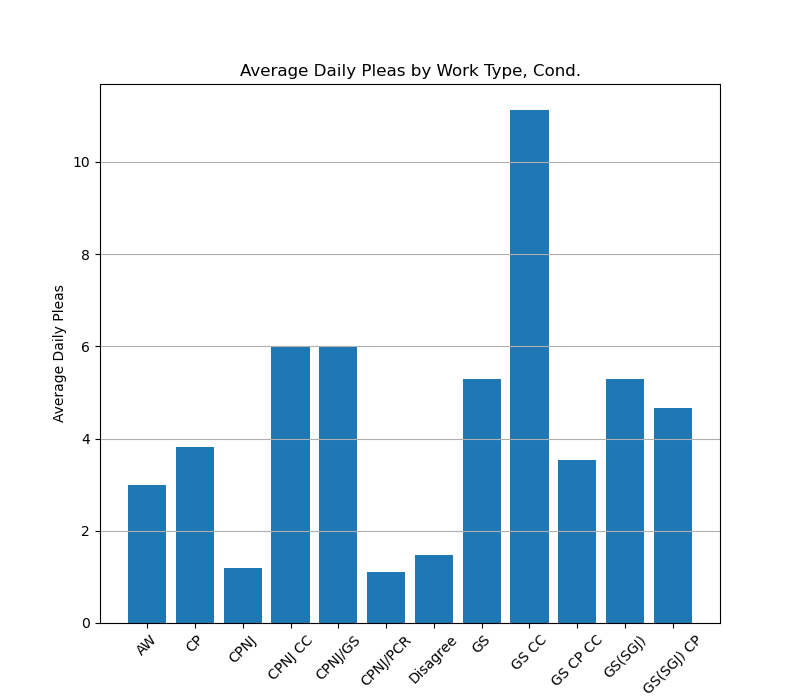
\includegraphics[width=0.75\textwidth]{../../../output/figures/Exploration/avg_pleas_by_worktype_cond.png}
    \caption{Average Pleas Processed per Day by Work Type, conditional on observing at least one sentencing event on that day. Disagree is when the sentencing and schedule data disagree, so we don't know what the work type is.}
    \label{fig-avg-plea-cond}
  \end{figure}

  \begin{figure}[H]
    \centering
    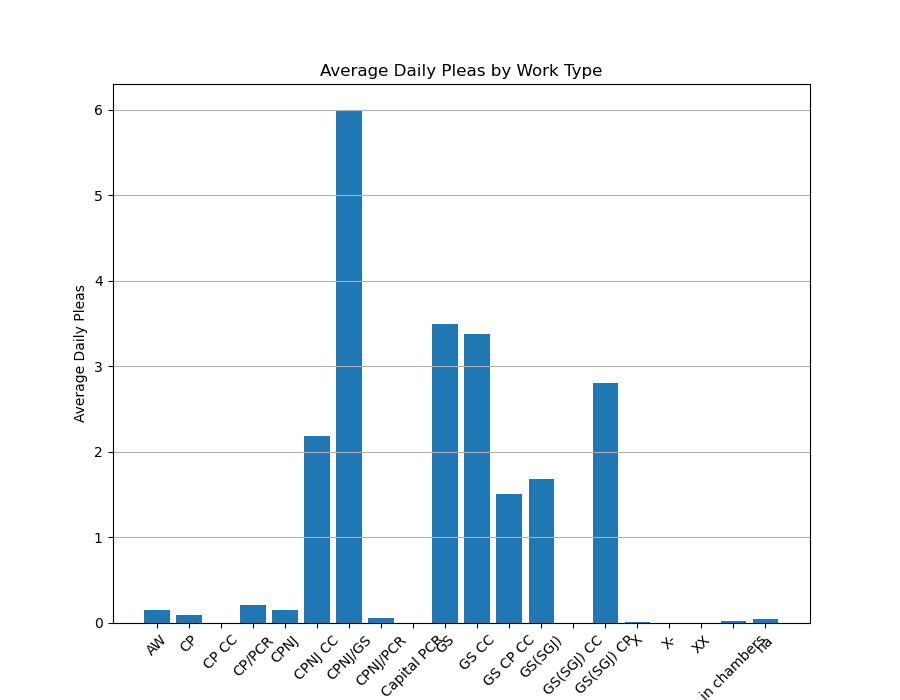
\includegraphics[width=0.75\textwidth]{../../../output/figures/Exploration/avg_pleas_by_worktype.png}
    \caption{Average Pleas Processed per Day by Work Type}
    \label{fig-avg-plea}
  \end{figure}

\section{Fraction GS and Fraction Clean Days by Judge}
  \begin{figure}[H]
    \centering
    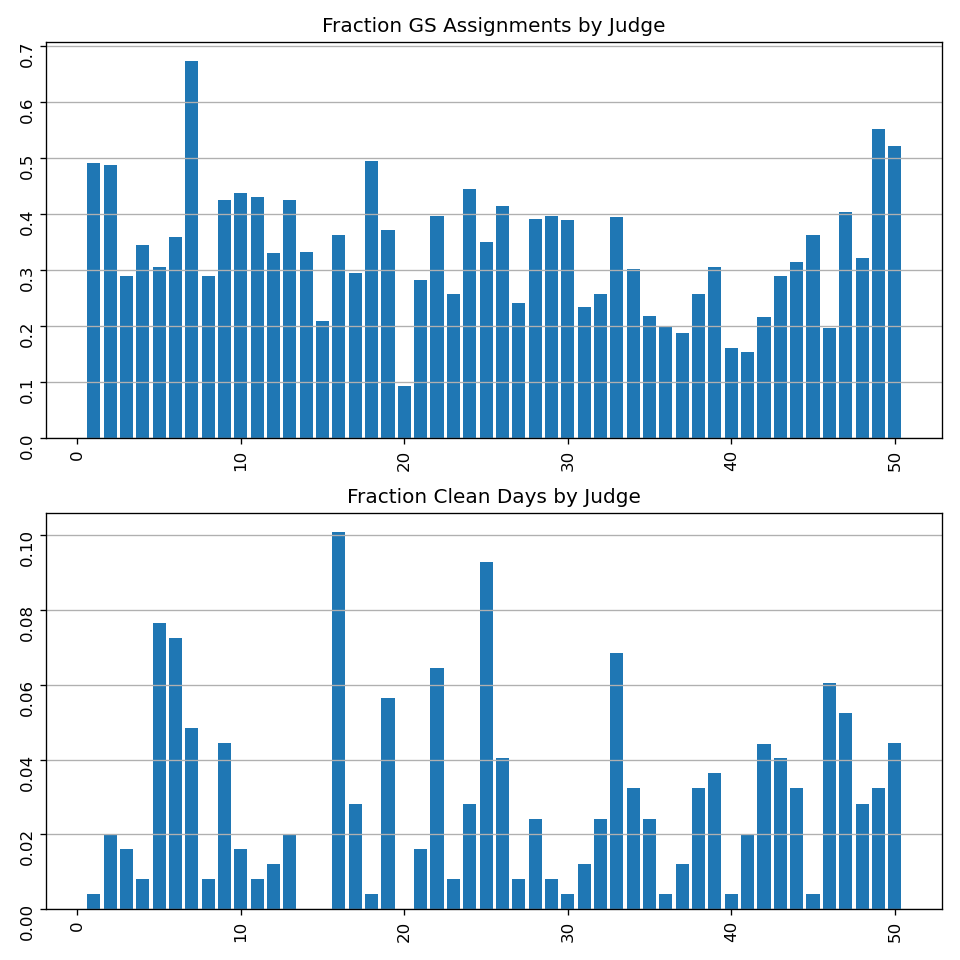
\includegraphics[width=0.85\textwidth]{../../../output/figures/Exploration/fraction_gs_clean.png}
    \caption{Fraction of GS days and Clean days by Judge}
  \end{figure}

\section{Distribution of Pleas Per Day by Broad Work Type}
  \begin{figure}[H]
    \centering
    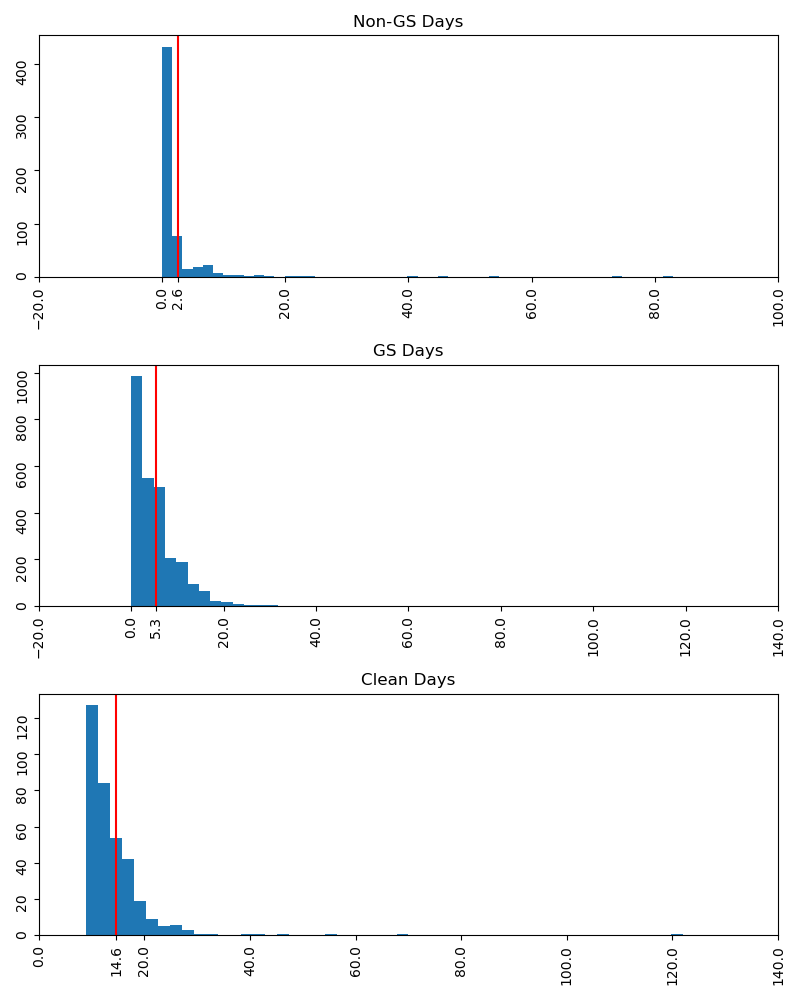
\includegraphics[width=0.75\textwidth]{../../../output/figures/Exploration/daily_plea_hist_by_broad_work_type.png}
    \caption{Distribution of the number of pleas processed per day, conditional on observing a sentencing event on that day.}
  \end{figure}

\end{document}
